\begin{myact}{1 page 184}
	\begin{enumerate}
		\item Dans l'expérience A, la lampe est toujours allumée avec le même éclat. Dans l'expérience B, elle clignote son éclat varie.\pause
		\item Dans les montages C et D, les LED sont placées en dérivation l'une par rapport àl'autre et dans des sens différents ; une résistance est également montée en série avec le générateur.\\
		Dans l'expérience C, la LED rouge est toujours allumée et la verte éteinte. Dans l'expérience D, elles clignotent l'une est éteinte quand l'autre est allumée.
		\item La tension aux bornes de la pile est constante, celle aux bornes du générateur très basse fréquence (GBF) varie.
		\item Si on branche la lampe sur une pile elle est tout le temps allumée, elle n'est pas clignotante.
		\item \ \begin{center}
			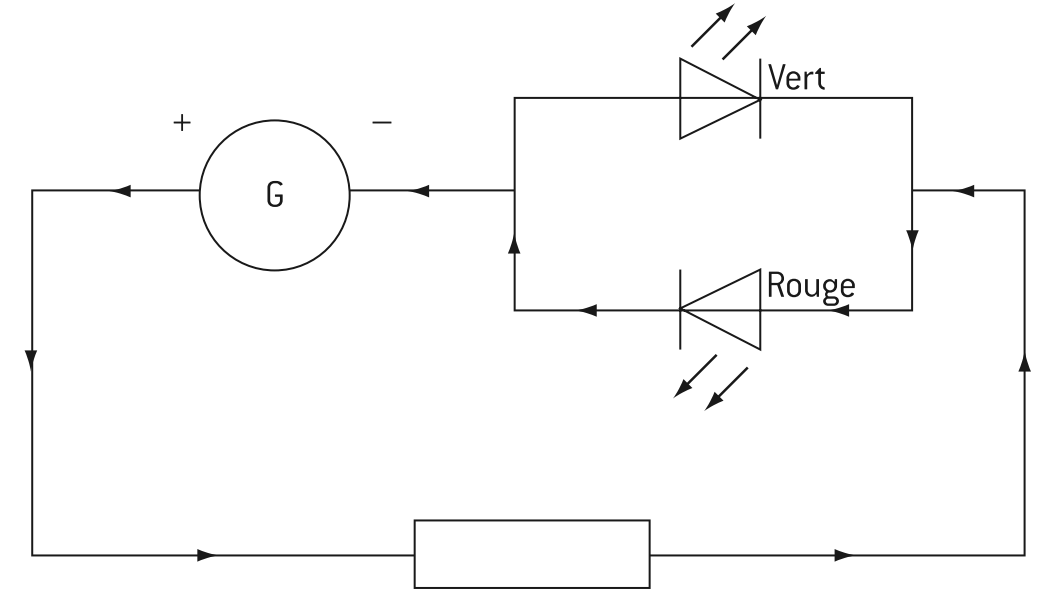
\includegraphics[scale=0.4]{act1_circuit}
		\end{center}
		\item Dans le circuit D le courant change régulièrement de sens.
		
	\end{enumerate}
\end{myact}